\section{Arkitektur}

\subsection{Systemarkitektur}
\noindent
Dette afsnit forklarer hvordan systemets toplevel arkitektur er opbygget.
Denne består af en bruger som interagerer med systemet gennem frontendapplikationen som skrives i WPF. States i denne applikation styres af Game modul som holder styr på hvor spilleren befinder sig, hvilke items der er samlet op og andre nyttige information som skal bruges gennem spillet.
Spillets backend benyttes primært til bruger authentication og som bindeled til databasen.
Databasen indeholder oplysninger om blandt andet brugere, de gemte spil og oplysninger om historien for de forskellige rum.

\begin{figure}[h]
\centering
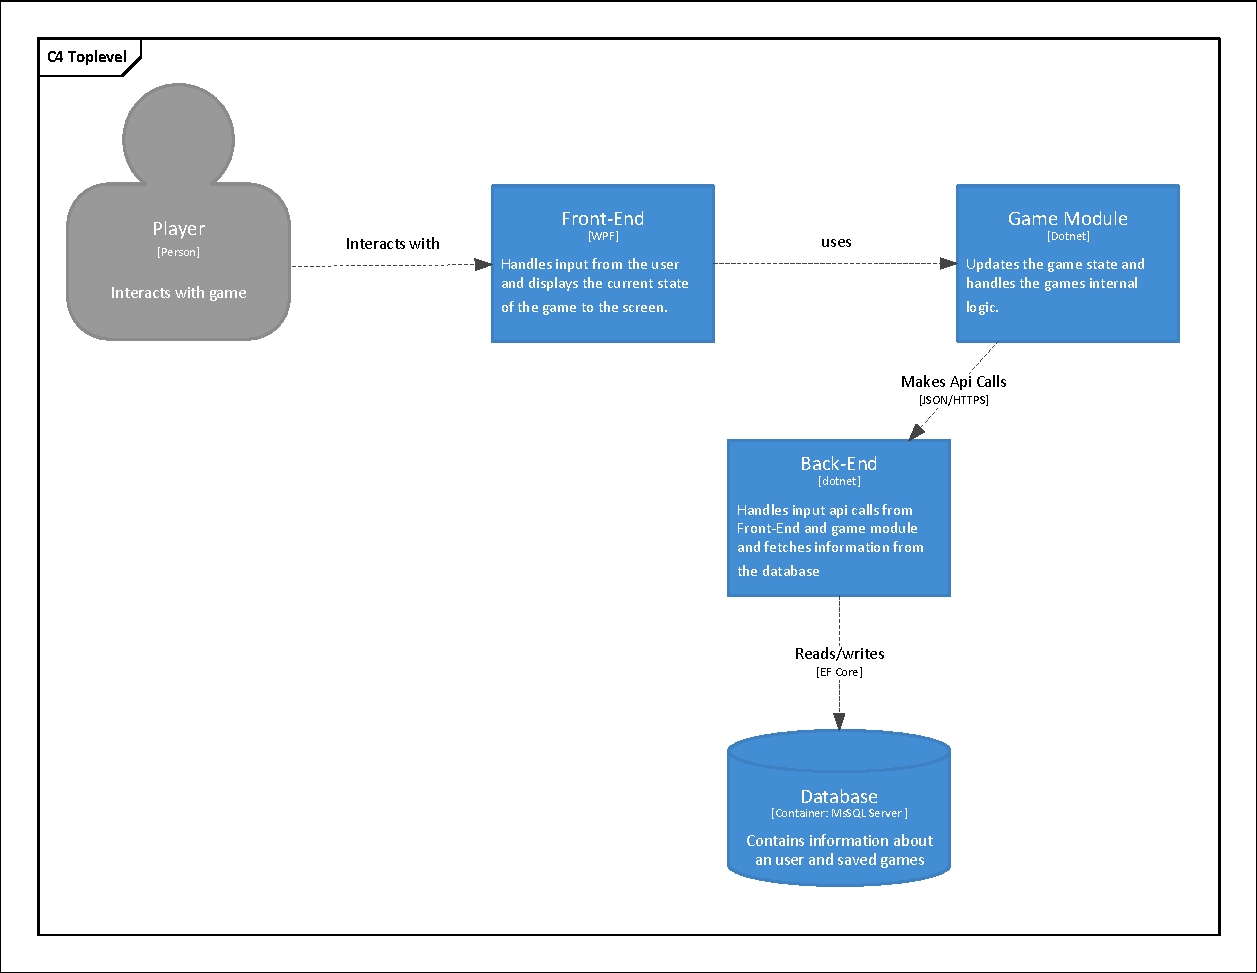
\includegraphics[width = \textwidth]{02-Body/Images/Arkitektur - C4TopLevel.pdf}
\caption{C4 Top-Level diagram for systemets arkitektur. Her ses et diagram for systemets Top-Level arkitektur, hvori der er skabt et overblik over hvilke moduler der er til stede i systemet og hvordan de kommunikere. Heri er der også tilføjet kommunikationsmetode for de forskellige forbindelser.}
\label{fig:Arkitektur-SD-SaveGame}
\end{figure}

